\documentclass[a4paper,titlepage]{article}

\usepackage{emp}
%\usepackage{cite}
\usepackage[pdftex]{graphicx}
\usepackage[english]{babel}
\usepackage[pdftex]{hyperref} %last

\DeclareGraphicsRule{*}{mps}{*}{}

%references setup
\hypersetup{colorlinks,
linkcolor=black,
citecolor=black,
filecolor=black,
urlcolor=black,
pdfauthor={Petter Ljungqvist}
}

% wide fields
\newenvironment{narrow}[2]{%
\begin{list}{}{%
\setlength{\topsep}{0pt}%
\setlength{\leftmargin}{#1}%
\setlength{\rightmargin}{#2}%
\setlength{\listparindent}{\parindent}%
\setlength{\itemindent}{\parindent}%
\setlength{\parsep}{\parskip}}%
\item[]}{\end{list}}

%\numberwithin{equation}{section}

\title{raytracer2}
\author{
	Petter Ljungqvist \and
	Hilkka Tamminen \and
	Anni Toppila}
\date{Last updated: \today}

\begin{document}
	\begin{empfile}
		\begin{empcmds}
			input metauml;
		\end{empcmds}
	
		\pagenumbering{alph}
		
		\maketitle
		
		\newpage
%\begin{fullwidth}
~\vfill
\thispagestyle{empty}
{\parindent0pt
\parskip15pt
%\setlength{\parindent}{0pt}
%\setlength{\parskip}{\baselineskip}
Copyright \copyright\ 2011--\the\year\ 
	{Petter Ljungqvist,
	Hilkka Tamminen,
	Anni Toppila}

\par Licensed under the Apache License, Version 2.0 (the "License");
   you may not use this file except in compliance with the License.
   You may obtain a copy of the License at

\hspace{15mm}\url{http://www.apache.org/licenses/LICENSE-2.0}. 

Unless required by applicable law or agreed to in writing, software
   distributed under the License is distributed on an \textsc{"as is" basis,
   without warranties or conditions of any kind}, either express or implied.
   See the License for the specific language governing permissions and
   limitations under the License.
}

%\end{fullwidth}
		
		
\begin{abstract}
	Raytracing is a method for generating images of three dimensional worlds. Artificial "rays" are shot from a camera (virtual eyepoint) trough every pixel of an image, and if the ray hits an object, the pixel's color is calculated from scene parameters at that intersection point. Any mathematical surface that can be intersected by a line can be rendered using raytracing.
	
	We have been focusing on rendering a realistic static image in this project. Performance has naturally been taken into account, but we have tried not to compromise the finale image. 
\end{abstract}
		
		\tableofcontents
		\addcontentsline{toc}{section}{Contents}
		
		\pagenumbering{arabic}
		\clearpage
		

		
\section{Instructions for compiling and use}

	The Raytracer has been tested to work on Aalto's Unix computers, but it should work on other platforms as well. For compiling simply go to the src folder and write the command \texttt{make}, and the program will compile to a file called raytracer.

	To run the program, simply write ./raytracer. The program will ask first for the scene file, then for the name of the file where you want to save the picture. The scene file is where all the information about the picture is stored, and for testing purposes you can use for instance \texttt{src/scene.txt}, which is uploaded in SVN. Alternatively, you can give the scene file as an argument to \texttt{raytracer} and then type in the picture name, or even give both as arguments eg 
	
	\texttt{./raytracer scene.txt pic.ppm}

	The program will read the scene file and create a picture with the given file name.

	%Note till Petter: lägg till nån fin bild hit?

	\begin{figure}
		\centering
		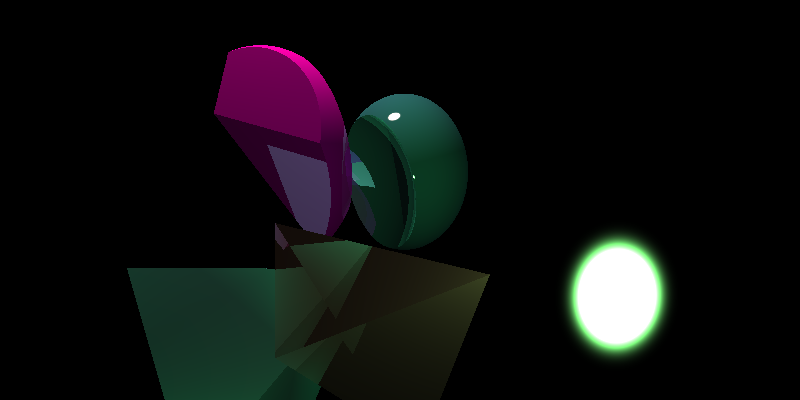
\includegraphics[width=\textwidth]{../img/pic.png}
		\caption{Example picture}
		\label{f:pic}
	\end{figure}
		
	
\section{Program architechture}

%	\emph{In this chapter you must describe the main architechture of your program. You \emph{must draw} clear diagrams of your program structure. You don't need to go in to the details, but this chapter should give the reader the idea of the architechture of your program. You must also tell, why you decided to use the architechture you used.}
	
	The project is built up of three main parts; a 3D-world, a rendering control and a input file reader.
	
	\subsection{World}

		The base of the architecture is a singleton class called \textbf{World}. World contains everything in the 3D-world. The abstract objects present in the world are called Thing and Light. The actual act of ray tracing happens in World as well. This means that the World doesn't need to be rebuilt for capturing an image from another position.

		The abstract class \textbf{Thing} is inherited from all objects which can be seen in the finale picture. The way they are seen depends on everything else (and itself) present in the world. The other type of objects that influence picture inherit the abstract class \textbf{Light}. Lights do not actually appear in the picture, they just contribute with light. Though the Lights aren't seen they can add some kind of Thing to World when they are created.

		Thing has a subclass called \textbf{SimpleThing} that is also a abstract class. SimpleThings are built up of only one material and colour. They can be combined in different manners with a subclass of SimpleThing called \textbf{CSG} (Combined Solid Geometry). That means that a CSG can be used in another CSG.

		A small UML-diagram of the world can be found in appendix \ref{f:world}.

	\subsection{Picture}
		The class \textbf{Picture} handles the capturing of the picture. It positions the camera, builds the raster and controls the rendering of the image. Picture is independent of the world it is possible to render different kinds of pictures.

	\subsection{Scene File}
		The scene file is read by the function FileReading::read(istraem file)and is described in appendix \ref{fileReading}.


		
\section{Data structures and algorithms}
	
%	In this chapter you must describe the data structures and algorithms used in your program. Dont't put your code here, but describe the data structures and algorithms using natural language (you can also add pictures).

	\begin{figure}
		\centering
		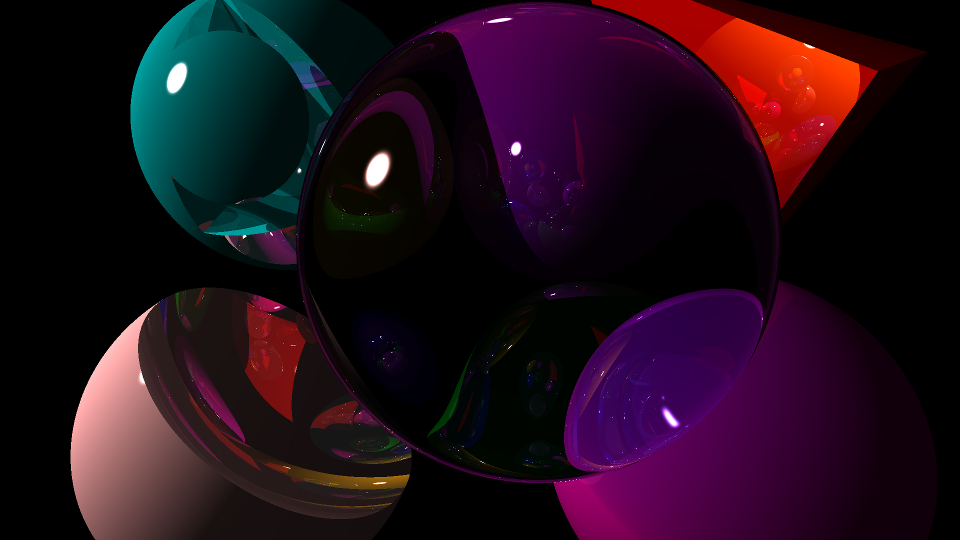
\includegraphics[width=\textwidth]{../img/shapes.png}
		\caption{Example picture}
		\label{f:shape}
	\end{figure}
	
	\subsection{Reading the Scene File}
		
		To build a world using the \emph{FileReading::read(std::istream file)} function a file (or other kind of stream) is needed. The reader reads the stream word by word and uses its \emph{sub}-functions to interpret the objects. All functions make use of the braces, \texttt{\{ \}}. The \texttt{constructive\_solid\_geometry} function uses the same function as the environment \texttt{thing} to add objects to itself. This recursion makes it possible to build complex \emph{CSG}s with many objects.

		The file reader is not necessary to build a World, it can be done through Worlds own functions (also used by the reader), but the scene file input is quite easy and has also helped us a lot with testing.
	
	\subsection{Building the World}
	
		The world is initialized at start-up. Then the different objects (the \emph{Thing}s and \emph{Light}s) in the world are built and added to the world after they are ready. The \emph{camera} is not part of the world, it just makes use of the worlds ray tracing capabilities. That means that many cameras can work on the same World object, and there is only one World per instance of the programme since the class is a singleton.

		The class World as it is built is not capable of moving its objects, just removing and adding new once. 
	
	\subsection{Prepering the Raster}
	
		The whole act of ray-tracing begins from the \emph{Picture} class. Picture had a \emph{Camera} that contains information about the set-up (position, direction, projection, angles, size etc.). The raster (the \emph{Ray}s) for the image is calculated by Picture and sent to the World instance using its function \emph{sendRay}. sendRay returns the colour generated by the ray. All the colours from the rays are stored in a class called \emph{PictureData}.
	
	\subsection{Ray Tracing} 
	
		The class Worlds function sendRay takes a Ray (contains two vectors, origin and direction). sendRay first loops through all the Things in the world and checks, with the Things checkRay function, whether the ray hits it or not. checkRay returns a lu (the length unit used throughout the project) which represents the distance the ray has to travel before hitting the object. From the point where the ray hits the object closest to its starting point (smallest value of the returned lu), if it hits any, three different rays are sent out. The shadow-ray, the reflection-ray and the refraction-ray. All these rays will return a colour and the final colour for send Ray to return is
		\begin{equation}
			c = i_{sh} c_{sh} + i_{rl} c_{rl} + i_{rr}c_{rr}
		\end{equation}
		where the $c$s are the colours and the $i$s the indices of the different phenomena. The $i$s should add up to one. The colour of three different rays are calculated somewhat differently:

		\subsubsection{Shadow-Ray}
			
			The shadow-ray represents the scattered lights. It is calculated for each light source in the world and all the colours added together. The colour contribution from each light source is calculated the following way:
			
			First a base colour is calculated by
			\begin{equation}
				c_{sh,b} = k\frac{c_{mat}c_{light}}{r^2}
			\end{equation}
			where $r$ is the distance to the light and $k$ is a coefficient that we have chosen to be 0.1. After that a ray from the the point to the light is checked for shading objects. If there are any not transparent objects in the way the or if the object itself is in the way of the light only the base colour is returned. If there aren't any objects in the way though a light colour is added to the base colour. The light colour is 
			\begin{equation}\label{e:cshl}
				c_{sh,l} = (1-k)\frac{c_{mat}c_{light}}{r^2}\mathbf{n}\cdot\mathbf{v}_l
			\end{equation}
			where $\mathbf{n}$ is the objects normal in the point and $\mathbf{v}_l$ is the unit vector pointing at the light source from the point.

			If the point is shaded by transparent objects the light in (\ref{e:cshl}) is shaded accordingly.
			
		\subsubsection{Reflection-Ray}
		
			The reflection-rays colour is generated by using the Worlds sendRay function from the point in the opposite direction of the incoming rays mirror image through the objects normal in the point.
		
		\subsubsection{Refraction-Ray}
		
			The refraction-ray goes into the object. The direction is calculated with the formula \cite{maol_sv}
			\begin{equation}\label{e:brytning}
				\frac{\sin \alpha_1}{\sin \alpha_2} = \frac{n_2}{n_1}.
			\end{equation}
			A ray is then sent in that direction through the object and from there it continues in again another direction determined with the same formula (\ref{e:brytning}). The part of the ray that goes through the object is shaded according to the objects materials properties:
			\begin{equation}
				c_{shade} = \left(c_{mat}k_{tansl}\right)^r c_{out ray}
			\end{equation}
			where $k_{transl}$ is the translucence coefficient and $r$ the distance the ray travels in the object. $c_{out ray}$ is the colour of the ray going out on the other side of the object. That colour is again calculated with Worlds sendRay.
		
	
	\subsection{Writing the Image to a File}
	
		At the end the PictureData can write out the colour raster to a simple \texttt{.ppm}-file.
	
	\subsection{Constructive Solid Geometry}
		
		The constructive solid geometry (or CSG) class combines two \emph{SimpleThing}s in one of three different combination types, union, intersection and complement union. A CSG has only one material. The materials in its SimpleThins are ignored. 

		The functions that the CSG needs to be able to calculate for these three types are
		\begin{description}
			\item[checkRay(ray:Ray\&,max:lu):lu] checks if a ray hits the object and returns the distance the ray has to travel before hitting it (returns a negative number if it doesn't hit it).
			\item[checkInnerRay(ray:Ray\&):lu] checks where a ray hits the back wall (ignoring the first surface) the same way as checkRay.
			\item[getNormal(position:Vect\&):Vect] returns a unit vector pointing out of the object. Always called for a point on the surface of the object.
			\item[wraps(position:Vect\&):bool] returns \emph{true} if the position is inside the object.
			\item[onSurfice(position:Vect\&):bool] returns \emph{true} if the position is on the surface of the object.
		\end{description}
		wraps and  onSurfice arn't ever true for the same position. For this a small $\Delta$ constant is used since doubles aren't very exact.
		
		\subsubsection{Union}
		
			In union combination the order of the tow objects doesn't matter. The functions listed above work as follows for unions.

			\begin{description}
				\item[checkRay] calls checkRay for both and returns the smaller positive one (returns a negative number if both ar enegative).
				\item[checkInnerRay] chacks checkInnerRay for both. Returns the positive one if only one is positive (a negative number if both are positive). If both are positive it checks if the smaller ones point is inside the other object (wraps), and if so returns the grater one, else the smaller.
				\item[getNormal] checks on which objects surface the position is (onSurface) an returns the normal (getNormal) from that object and point.
				\item[wraps] returns \emph{true} if wraps is true for either object.
				\item[onSurfice] returns \emph{true} if true fore one of the objects and not inside (wraps) the other object.
			\end{description}
		
		\subsubsection{Intersection}
		
			Intersection is the space occupied by both objects.

			\begin{description}
				\item[checkRay] if positive for both it returns the smaller one.
				\item[checkInnerRay] if positive for both it returns the greater on (with some tweaks for non convex objects).
				\item[getNormal] checks on which objects surface the position is (onSurface) an returns the normal (getNormal) from that object and point.
				\item[wraps] returns \emph{true} if true for both objects.
				\item[onSurfice] returns \emph{true} if true fore one of the objects and inside (wraps) the other object.
			\end{description}
		
		\subsubsection{Complement Union}
		
			Intersection is the space occupied by the first (left) object, but not the second (right).

			\begin{description}
				\item[checkRay] if positive for left it checks if that point is inside right. If so it returns rights checkInnerRay else lefts checkRay. If negative for left if returns a negative number. Except when the ray starts inside left, then rights inner ray is tested and if that point is inside left as well it returns rights inner ray.
				\item[checkInnerRay] if positive for left it checks if that point is inside right. If so it returns rights checkRay else lefts chaeckInnerRay. If negative for left if returns a negative number. Except when the ray starts inside left, then lefts inner ray is tested and if that point is not inside right it returns lefts inner ray.
				\item[getNormal] checks on which objects surface the position is (onSurface) an returns the normal from left if it is left and -normal from right else.
				\item[wraps] returns \emph{true} if true left and false for right.
				\item[onSurfice] returns \emph{true} if true fore left and not inside right or true for right and inside left.
			\end{description}
		
\section{Known bugs}

%	In this chapter you must tell all known bugs in your code. You must also tell what could have been done better.


%	If the assistant finds bug(s) in your code that you haven't mentioned, it is very bad thing and your points will be decreased. And if your code segfaults, it is even worse and your points will be decreased more...

	\begin{itemize}
		\item The ray tracer isn't counting reflections, so there is a possibility of infinite reflections (e.g. a CSG of a sphere and a smaller complement inside it). This is not hard to fix, has just not been done.
		\item The ThingPlane (created with \texttt{plane} in the \texttt{special\_thing} environment) is onesided. So it works poorly as a transparent surface. (Not actually a bug.)
	\end{itemize}

		
\section{Tasks sharing and schedule}

%	In this chapter you must tell how the task sharing and communication inside the group worked. You must also tell the real schedule and amount of work done by each group member. You are also encouraged to describe the amount of work of each different part you your project. (planning, implementation of different areas of project, testing and documentation etc.)


%	Think and tell also, if you could have shared tasks better. What went wrong compared to the schedule of your original plan and why.
	
The group communicated via e-mail and weekly meetings. The meetings were convenient for keeping everybody up to date on the latest progress and possible changes to how things were done.

After the plan was presented to the assistant in the beginning of the project, a more detailed schedule was made. Milestones were set up for every week and the work was divided and shared with more detail. By November 17th we wanted to be able to create a picture with just spheres, a week later spheres and some other shapes with lights as well, and then by the 30th all the basic functionalities were to work. A shared document was made on Google Docs that we were supposed to tick off sections in every time we finished something.

In practice the project advanced in a different order and for the most part ahead of time. Very quickly we had pictures with spheres, lights, constructive solid geometry, reflections and translusans. The freely movable camera was finished around the time scheduled, while the file reading function was worked on later than we had thought.

Most of the workload was done by Petter, who handled general things such as creating the header files and the file dependencies, but who also did most of the work in World, Light, Thing, Sphere, CSG... Anni handled the camera and its movements and writing the data out to a file. Hilkka made part of Material, Colour and Vect classes and wrote the first version of the file reading function, which Petter then improved and added error handling to.

Testing of each part was done individually and so well that there were no bigger problems when fitting them together. The testing was not planned in detail in advance, but that didn't cause any problems.

Documentation was done together: each group member wrote more or less the same amount.
		
\section{Differences to the original plan}
	
%	In this chapter you must tell what is done in different way that was originally planned and why.

%	Do you think your plan was good enough, super, or should you have planned your program better?

The original plan turned out to be quite good and no mayor changes where needed. There were naturally quite a bit of stuffing added in the implementations stage, but the main idea stayed the same. Our clear original plan helped us to understand each other and what we wanted from the project and made it easier to work towards a common goal.
	
		\clearpage
		\pagenumbering{roman}
		\appendix
		
		
%\section{References}

%	In this chapter you must tell all the references you have used during your project.
	
	
	
	%\renewcommand\refname{}
	\addcontentsline{toc}{section}{References}
	\bibliography{raytracer_doc}{}
	\bibliographystyle{plain}
	
	\href{http://www.cplusplus.com/reference/}{C++ : Reference \emph{online} \texttt{http://www.cplusplus.com/reference/}}

		
\section{Detailed Instructions for Writing a Scene File \label{a:scene} \label{fileReading}}

All the parameters of the picture are defined in a so-called scene file. That means that all information about the objects, the lights, the camera and the picture size should be found there, structured in a certain way.

The scene file is divided into main sections, called \texttt{thing}, \texttt{special\_thing}, \texttt{light}, \texttt{camera} and \texttt{picture\_size}, containing information about the respective subjects. All sections are defined using curly brackets \texttt{\{ \}}. The brackets must not touch the other words meaning there must always be at least a white space between the other words and the brackets. The order of the sections or the order of the information within the sections are not important.

Indentation does not matter, but is advisable for clarity. Everything should be in lowercase, except the type parameter in constructive solid geometry. Commenting is possible, and it is done by writing \texttt{//} before the comment. As in C++, the rest of the line after the \texttt{//} will be ignored. There is a difference though; here it is compulsory to have a white space between the \texttt{//} and the text. 

In the \texttt{thing} section, an unlimited amout of objects can be declared. Each new sections starts with the name of the type of object: \texttt{sphere}, \texttt{tetrahedron}, \texttt{cylinder} or \texttt{constructive\_solid\_geometry}. So far the thing section would look like this:

\begin{verbatim}
thing {
     sphere {
     }
     sphere {
     }
     tetrahedron {
     }
     cylinder {
     }
     constructive_solid_geometry {
     }
}
\end{verbatim}

A sphere must have a position, a radius and a material section containing the material values and the colour. All values are defined by writing first the name of the value, then the value itself, e.g. \texttt{radius 3.5}. Position and colour, which have several values, are also defined on one line: position in the form \texttt{position x y z} and colour by \texttt{colour r g b}.

The material section should have the \texttt{reflection}, \texttt{refraction}, \texttt{scattering}, \texttt{translusans}, refractive index (written together: \texttt{refractive\_index}) and the \texttt{colour}. Note that in order the be realistic, the values for reflection, refraction and scattering need to add up to 1.0. Unless they are all given as 0, the program will make sure this law is fulfilled. All the values in the material section should be in the interval [0, 1]. The only exception are the colour values for lamps, which can be significantly bigger.

The \texttt{sphere} section will then look like this:

\begin{verbatim}
sphere {
     material {
         reflection 0.2
         refraction 0.6
         scattering 0.2
         translusans 0.5
         refractive_index 0.2
         colour 0.1 0.9 1
     }
     position 1 2 1
     radius 1.5
}
\end{verbatim}

For tetrahedrons, the material is defined the same way as for the sphere, but the position and size are defined by giving the coordinates of the shape's corners in space. The \texttt{tetrahedron} section would thus look like this: 

\begin{verbatim}
tetrahedron {
    material {
      ...
    }
    vect1 1 2 3
    vect2 2 3.5 3
    vect3 3 2 3.3
    vect4 4 2 3
}
\end{verbatim}

Cylinders are made the same way. They are created with \texttt{cylinder} and their parameters are \texttt{end\_1} and \texttt{end\_1} for the ends and \texttt{radius}. eg:

\begin{verbatim}
cylinder {
    material {
      ...
    }
    end_1 14 -1 0
    end_2 0 1 0
    radius 1
}
\end{verbatim}

Constructive solid geometry is a little more complicated. In this program, the CSGs are always made up of two SimpleThings, i.e. spheres, tetrahedrons or even other CSGs. The type of interaction between the Things is defined as union (\texttt{U}), intersection (\texttt{I}) or complement (\texttt{C}). CSGs also need a material. The Things are called \texttt{left} and \texttt{right}, but the names have no significance. Note: it is up to the user to make sure the two parts of the CSG intersect.

The \texttt{constructive\_solid\_geometry} section will have a \texttt{left} and a \texttt{right} section. These will include a Thing definition. Material definitions for left and right are not needed and can be left out. The \texttt{constructive\_solid\_geometry} section will then look like this:

\begin{verbatim}
constructive_solid_geometry {
    left {
        sphere {
            position 2 2 1
            radius 1
        }
    }
    right {
        constructive_solid_geometry {
            left {
                sphere {
                    position 1 2 1
                    radius 1.5
                }
            }
            right {
                sphere {
                    position 2 2 2
                    radius 1
                }
            }
            type U
        }
    }
    material {
        ...
    }
    type I
}
\end{verbatim}

The \texttt{special\_thing} environment have thing which can not be used in a \texttt{constructive\_solid\_geometry}.

\texttt{plane} is a infinite plane. It is constructed from three points in the plan and one (nr. 4) the shows which site is the top of the plane. The plane should always have its top towards the camera, so a good practice is the use the cameras position as the fourth point. Using transparent surfaces is not recommended, since the plane is only onesided. Example of plane construction:

\begin{verbatim}
special_thing {
     plane {
         mateial {
             ...
         }
         point 1 1 2 3
         point 2 3 2 1
         point 3 1 1 0
         point 4 0 0 0
     }
}
\end{verbatim}

The \texttt{light} section works the same way as the Thing section; all the Light objects are defined there for each type (\texttt{lamp} or \texttt{spotlight}). As explained before, the difference between the two types of Light is that \texttt{spotlight} is a point light, it is only just the light source, whereas \texttt{lamp} has a sphere around the light source to give it a more natural look.

Spotlights are defined by simply giving the colour and the position. For lamps, the size of the sphere is also given. Remember that for lights the colour values can be much greater than 1. The \texttt{light} section will then look something like this:

\begin{verbatim}
light {
    lamp {
        colour 200 300 200
        position 3 4.5 6
        size 1
    }
    lamp {
        colour 180 30 150
        position 1 2.5 6
        size 3
    }
    spotlight {
        colour 100 200 250
        position 1 3.5 6
    }
}
\end{verbatim}

Everything related to the camera is described in the \texttt{camera} section. The camera is defined by its position, which direction it shoots at, which direction is up, how wide is the angle of the shoot, and what type of projection is it. The angles are given in degrees in x and y directions, and the type of  projection is given as a character: 1 means a polar coordinate system, anything else mean a cartesian coordinate system. The \texttt{camera} section does not have running numbers, and looks for instance like this:

\begin{verbatim}
camera {
    position 2.05 3.10 4.2
    centre 0.0000 2.1 4.5
    up 3.2000 9.5 3.3
    projection i
    angle_x 45.0
    angle_y 90
}
\end{verbatim}

The last part of the scene file is the picture size. It is in its own section, like everything else, and is quite simple:

\begin{verbatim}
picture_size {
    x_max 1500
    y_max 1000
}
\end{verbatim}
The scene file must end with the word \texttt{end}.
		
		%\clearpage
		
			\begin{figure}
				\section{World UML-diagram} 
				\label{f:world}
				\begin{narrow}{-40pt}{-40pt}
					\centering
					
\begin{emp}[classdiag](0,0)

	iClass.foreColor := (1, 1, 1);
	iAbstractClass.foreColor := (1, 1, 1);
	iClass.iName.iFont.scale := .8;
	iClass.iAttributeStack.iPict.iFont.scale := .8;
	iClass.iMethodStack.iPict.iFont.scale := .8;
	iAbstractClass.iName.iFont.scale := .8;
	iAbstractClass.iAttributeStack.iPict.iFont.scale := .8;
	iAbstractClass.iMethodStack.iPict.iFont.scale := .8;
	
	Class.World("World")
		(
			"-static inst:World*",
			"-things:list<Thing*>",
			"-lights:list<Light*>"
		)(
			"+static Instace(): World*",
			"+addThing(thing:Thing*)",
			"+removeThing(thing:Thing*)",
			"+addLight(light:Light*)",
			"+sendRay(ray:Ray,thing:Thing*):Colour",
			"+worldColour(thing:Thing*,position:Vect&,normal:Vect&):Colour",
			"+getThing(position:Vect&):Thing*",
			"+Release()"
		);
		classStereotypes.World("<<singleton>>");
		
% 	Class.Pict("Picture")
% 		(
% 			"-camera:Camera",
% 			"-picture:PictureData"
% 		)(
% 			"+Picture()",
% 			"+capture():PictureData",
% 			"+getPicture():PictureData"
% 		);

	AbstractClass.Li("Light")
		()(
			"+virtual illumination(position:Vect&):LightRay",
			"+virtual getPosition():Vect",
			"+virtual addToWorld()"
		);
		
	Class.SpLi("some Lights")
		(	
			"-properties"
		)(
			"+Lights()",
			"+illumination(position:position:Vect&):LightRay",
			"+getPosition():Vect",
			"+addToWorld()"
		);
		
	AbstractClass.Thing("Thing")
		(
		)(
			"+~Thing()",
			"+virtual checkRay(ray:Ray&,max:lu):lu",
			"+checkRay(ray:Ray&):lu",
			"+virtual checkInnerRay(ray:Ray&):lu",
			"+virtual getMaterial(ray:Ray&):Material",
			"+virtual getMaterial(position:Vect&):Material",
			"+virtual getColour(ray:Ray&):Colour",
			"+virtual getColour(position:Vect&):Colour",
			"+virtual getNormal(position:Vect&):Vect",
			"+virtual wraps(position:Vect&):bool",
			"+virtual onSurfice(position:Vect&):bool"
		);
		
	Class.Things("some Things")
		(
			"-properties"
		)(
			"+Things(properties)",
			"+checkRay(ray:Ray&,max:lu):lu",
			"+checkInnerRay(ray:Ray&):lu",
			"+getMaterial(ray:Ray&):Material",
			"+getMaterial(position:Vect&):Material",
			"+getColour(ray:Ray&):Colour",
			"+getColour(position:Vect&):Colour",
			"+getNormal(position:Vect&):Vect",
			"+wraps(position:Vect&):bool",
			"+onSurfice(position:Vect&):bool"
		);
		
	AbstractClass.SThing("SimpleThing")
		(
			"-material:Material"
		)(
			"+SimpleThing(mat:Material)",
			"+getMaterial(ray:Ray&):Material",
			"+getMaterial(position:Vect&):Material",
			"+getColour(ray:Ray&):Colour",
			"+getColour(position:Vect&):Colour"
		);
		
	Class.Sph("some SimpleThings")
		(
			"-properties"
		)(
			"+SimpleThings(properties)",
			"+checkRay(ray:Ray&,max:lu):lu",
			"+checkInnerRay(ray:Ray&):lu",
			"+getNormal(position:Vect&):Vect",
			"+wraps(position:Vect&):bool",
			"+onSurfice(position:Vect&):bool"
		);
		
% 	Class.Tetra("Tetrahedron")
% 		(
% 			"-p[4]:Position",
% 			"-planes[4]:pair<Position,Position>"
% 		)(
% 			"+Tetrahedron(a:Position,b:Position,c:Position,d:Position)",
% 			"+checkRay(ray:Ray,max:lu):lu",
% 			"-getNormal(ray:Ray):Position"
% 		);
	
	Class.csg("CSG")
		(
			"-left:SimpleThing*",
			"-right:SimpleThing*",
			"-binOp:char"
		)(
			"+CSG(mat:Material)",
			"+CSG(mat:Material,l:SimpleThing*,b:char,r:SimpleThing)",
			"+~CSG()",
			"+setLeft(thing:SimpleThing)",
			"+setRight(thing:SimpleThing)",
			"+setBinOp(b:char)",
			"+checkRay(ray:Ray&,max:lu):lu",
			"+checkInnerRay(ray:Ray&):lu",
			"+getNormal(position:Vect&):Vect",
			"+wraps(position:Vect&):bool",
			"+onSurfice(position:Vect&):bool"
		);
		
% 	Pict.s = World.n + (0, 20);
	Li.nw = World.ne + (20, 0);
	SpLi.nw = Li.sw + (0, -20);
	Thing.nw = World.sw + (0, -20);
	SThing.n = Thing.s - (0, 20);
	csg.nw = SThing.ne + (40, 0);
	Sph.n = SThing.s - (0, 20);
	Things.nw = Thing.ne + (40, 0);
%	csg.top = (Things.bottom - 20);
% 	Tetra.nw = Sph.ne + (10, 0);
	drawObjects(World, Li, SpLi, Thing, SThing, Sph, csg, Things);
	

	link(dependency)(pathVertical(World.s, Thing.top));
 	link(inheritance)(SThing.n -- Thing.s);
 	link(inheritance)(Sph.n -- SThing.s);
 	link(dependency)(rpathHorizontal(Li.w, World.right));
 	link(inheritance)(rpathVertical(Li.s, SpLi.top));
 	link(aggregationUni)(pathHorizontal(SThing.e, csg.left));
 	link(inheritance)(pathHorizontal(Things.w, Thing.right));
	
	
%	link(aggregation)(pathStepX(.5[World.nw, World.n], .5[World.n, World.ne], 20));
%	link(association)(Pict.s -- World.n);
%	link(inheritance)(.5[Tetra.n, Tetra.nw] -- .5[SThing.s, SThing.se]);

\end{emp}


				\end{narrow}
			\end{figure}
			
		% 	\begin{figure}
		% 		\centering
		% 		
\begin{emp}[classdiag](0,0)

	iClass.foreColor := (1, 1, 1);
	iAbstractClass.foreColor := (1, 1, 1);
	iClass.iName.iFont.scale := .8;
	iClass.iAttributeStack.iPict.iFont.scale := .8;
	iClass.iMethodStack.iPict.iFont.scale := .8;
	iAbstractClass.iName.iFont.scale := .8;
	iAbstractClass.iAttributeStack.iPict.iFont.scale := .8;
	iAbstractClass.iMethodStack.iPict.iFont.scale := .8;
	
	Class.Col("Colour")
		(
			"-R:size_t",
			"-G:size_t",
			"-B:size_t"
		)(
			"+Colour(R:size_t,G:size_t,B:size_t)",
			"+Colour(c:Colour)",
			"+operator=(c:Colour):Colour",
			"+operator+(c:Colour):Colour",
			"+operator-(c:Colour):Colour",
			"+operator*(c:Colour):Colour",
			"-Colour()"
		);
		
	Class.Cam("Camera")
		(
			"+pos:Position",
			"+centre:Position",
			"+up:Position",
			"+projection:char",
			"+angle_x:float",
			"+angle_y:float"
		)();
		classStereotypes.Cam("<<struct>>");
		Cam.info.iMethodStack.top := 0;
		Cam.info.iMethodStack.bottom := 0;
		
	Class.PD("PictureData")
		(
			"-res_x:size_t",
			"-res_y:size_t",
			"-data:vector<vector<Colour>>"
		)(
			"+PictureData()"
		);
		
	Class.lu("lu")
		(
			"float"
		)();
		classStereotypes.lu("<<typedef>>");
		lu.info.iMethodStack.top := 0;
		lu.info.iMethodStack.bottom := 0;
		
	Class.Pos("Position")
		(
			"+x:lu",
			"+y:lu",
			"+z:lu"
		)();
		classStereotypes.Pos("<<struct>>");
		Pos.info.iMethodStack.top := 0;
		Pos.info.iMethodStack.bottom := 0;
		
	Class.Mat("Material")
		(
			"-reflection:float",
			"-refraction:float",
			"-absorbtion:float",
			"-tanslu:float",
			"-col:Colour"
		)(
			"+Material()"
		);
		
	Class.Ray("Ray")
		(
			"+orgin:Position",
			"+diretion:Position"
		)();
		classStereotypes.Ray("<<struct>>");
		Ray.info.iMethodStack.top := 0;
		Ray.info.iMethodStack.bottom := 0;
		
	Class.LRay("LightRay")
		(
			"+ray:Ray",
			"+cal:Colour"
		)();
		classStereotypes.LRay("<<struct>>");
		LRay.info.iMethodStack.top := 0;
		LRay.info.iMethodStack.bottom := 0;

	Mat.nw = Col.ne + (20, 0);
	Cam.nw = Mat.ne + (20, 0);
	PD.nw = Col.sw - (0, 20);
	Pos.nw = Mat.sw - (0, 20);
	lu.nw = Pos.ne + (20, 0);
	Ray.nw = Pos.sw - (0, 20);
	LRay.nw = Ray.ne + (20, 0);
	drawObjects(Col, Cam, PD, Pos, lu, Mat, Ray, LRay);

\end{emp}


		% 		\caption{Structs \label{f:struct}}
		% 	\end{figure}
		
	\end{empfile}
\end{document}
